\subsection{Messergebnisse und Auswertung}
\subsubsection{Bestimmung der Verdet-Konstante}
Für jede Spannung $I$ wurde $N=4$ mal der entsprechende Winkel $\alpha_i$ gemessen. Der Fehler einer Einzelmessung des Winkels wurde auf
\begin{equation}
  s_{\alpha_i} = 0.2^\circ
\end{equation}  % TODO Fehler auf Strom
geschätzt. Es wird zunächst der Mittelwert der Winkel gebildet:
\begin{equation}
  \alpha = \frac{1}{N} \sum_{i=1}^{N} \alpha_i, \qquad s_{\alpha} = \frac{s_{\alpha_i}}{\sqrt{N}}
\end{equation}
Der Fehler auf den Strom wurde auf $s_I = 0.1$\,A geschätzt.\\
Die Spannungen und gemittelten Winkel werden nun mit einer Geraden gefittet:
\begin{equation}
  \alpha(I) = a + b \cdot I
\end{equation}
Die Werte und der Fit sind in \autoref{img:faraday} dargestellt. Die Kurvenanpassung ergab folgende Werte:
\begin{equation}
\begin{split}
  \label{eq:faraday:params}
  a &= (-0.28 \pm 0.06)\,{}^\circ \\
  b &= (2.5769 \pm 0.0199)\,\frac{{}^\circ}{\text{A}}
\end{split}
\end{equation}
\begin{figure}[H]
\begin{center}
  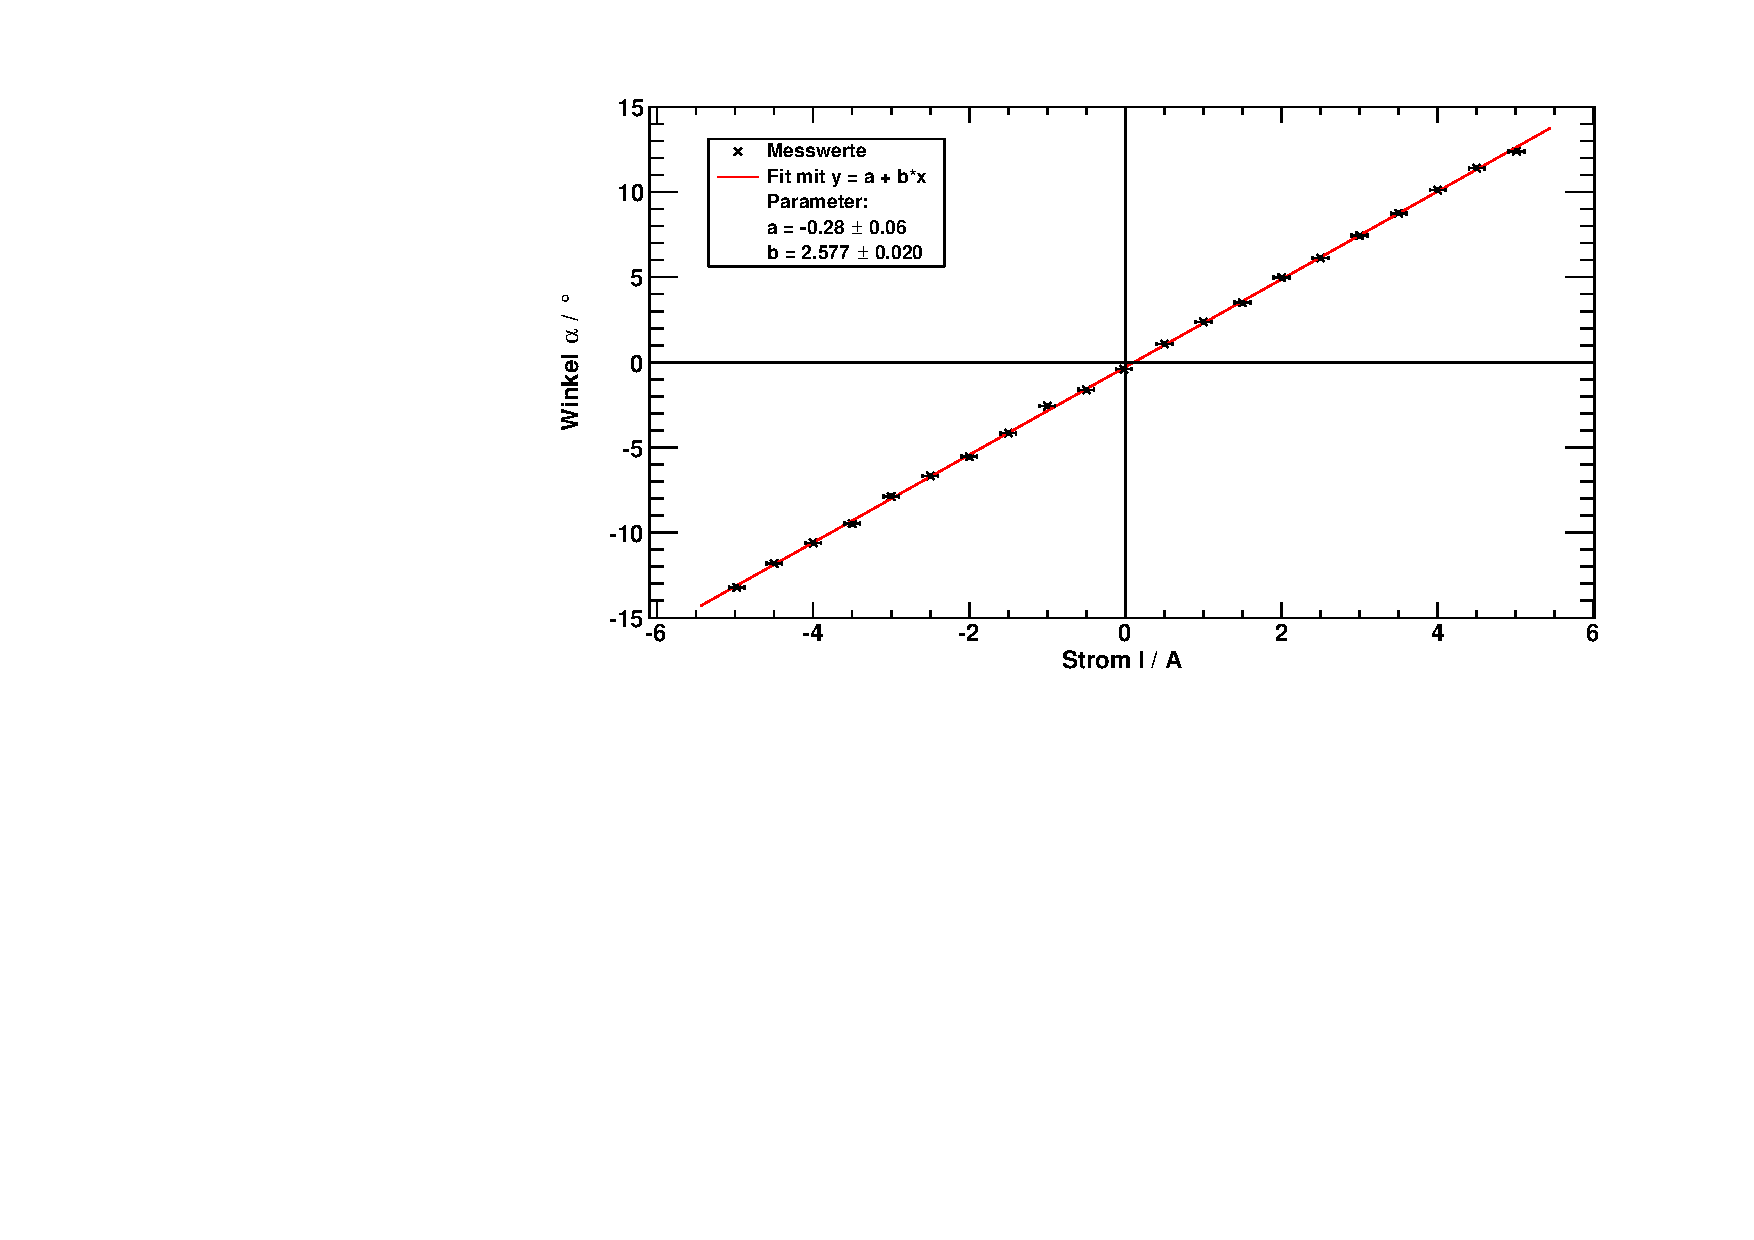
\includegraphics[width=\textwidth]{../img/faraday.pdf}
  \caption{Winkel $\alpha$ in Abhängigkeit des Stroms $I$ mit Fit einer Geraden.}
  \label{img:faraday}
\end{center}
\end{figure}
Mit \autoref{eq:verdet} wird nun die Verdet-Konstante $V$ berechnet:
\begin{equation}
  \label{eq:eval:verdet}
  V = \frac{b}{2556}, \qquad s_V = \frac{s_b}{2556}
\end{equation}
\begin{equation}
  V = (1.009 \pm 0.008) \cdot 10^{-3}\,\frac{{}^\circ}{\text{A}}
\end{equation}

\paragraph{Vergleich mit der Herstellerangabe}
Die Verdet-Konstante rechnet man folgendermaßen in $\frac{\text{min}}{\text{Oe}\cdot \text{cm}}$ um:
\begin{equation}
  1\,\frac{{}^\circ}{\text{A}} = \frac{60\cdot 79.58}{100}\,\frac{\text{min}}{\text{Oe}\cdot \text{cm}}
\end{equation}
Es folgt für den berechneten Wert:
\begin{equation}
  V = (0.0482 \pm 0.0004)\,\frac{\text{min}}{\text{Oe}\cdot \text{cm}}
\end{equation}
Der Hersteller gibt:
\begin{equation}
  V^{\text{Herst.}} = 0.05\,\frac{\text{min}}{\text{Oe}\cdot \text{cm}}
\end{equation}
als Wert an. Der gemessene Wert stimmt innerhalb des $5-\sigma$-Intervalls mit der Herstellerangabe überein, vorausgesetzt dass diese keinen Fehler 
besitzt. Betrachtet man die Rundung, so kann die Herstellerangabe zwischen $(0.045 \leq 0.05 < 0.055)\,\frac{\text{min}}{\text{Oe}\cdot \text{cm}}$ liegen. 
Mit diesem Fehler von $0.005\,\frac{\text{min}}{\text{Oe}\cdot \text{cm}}$  würden die beiden Werte innerhalb ihrer Fehler übereinstimmen.

\paragraph{Vergleich mit einer idealen Zylinderspule}
Hätte man anstelle einer realen Zylinderspule eine ideale Spule ($H^{\text{ideal}} = \frac{N \cdot I}{l}$) angenommen, 
so berechnet sich der Drehwinkel nach \autoref{eq:faraday} mit:
\begin{equation}
  \label{eq:alpha:ideal}
  \alpha = V \cdot N \cdot I \quad \Rightarrow b = V \cdot N \Leftrightarrow V = \frac{b}{N}
\end{equation}
Es ergibt sich nun äquivalent zu \autoref{eq:eval:verdet} eine Verdet-Konstante von:
\begin{equation}
  V^{\text{ideal}} = (0.716 \pm 0.006) \cdot 10^{-3}\,\frac{{}^\circ}{\text{A}} = (0.0342 \pm 0.0003)\,\frac{\text{min}}{\text{Oe}\cdot \text{cm}}
\end{equation}
Sie weicht sehr weit von dem Wert der realen Spule und der Herstellerangabe ab, weshalb die Näherung einer idealen Spule nicht gerechtfertigt ist. \\
Des Weiteren sieht man an \autoref{eq:alpha:ideal}, dass die in den Grundlagen (Kapitel \ref{subsub:alpha}) berechnete Konstante 
$c = 2554.85$ eine effektive Windungsanzahl darstellt, die eine ideale Spule besitzen müsste, um das Licht um den gleichen Winkel zu drehen.
\subsubsection{Bestimmung von 2\textepsilon}
Der Winkel $\alpha$ der Stellungen "`innen maximal dunkel"' ($\alpha_i$) und "`außen maximal dunkel"' ($\alpha_a$) wurde 
jeweils $N = 4$ mal gemessen. Der Fehler einer Einzelmessung wurde auf $s_{\alpha_i} = 2^\circ$ geschätzt. 
Es wird der Mittelwert gebildet
\begin{equation}
  \alpha = \frac{1}{N} \sum_{i=1}^{N} \alpha_i, \qquad s_{\alpha} = \frac{s_{\alpha_i}}{\sqrt{N}}
\end{equation}
und die Differenz der beiden Winkel gebildet:\footnote{Die Fehler der beiden Winkel sind gleich ($s_{\alpha_a} = s_{\alpha_b}$), weil hier der 
Messfehler und nicht die Standardabweichung der Messwerte benutzt wurde, da die Standardabweichungen mit dem Fehler $s_\alpha$ übereinstimmen.}
\begin{equation}
  2 \epsilon = \alpha_a - \alpha_i, \qquad s_{2\epsilon} = \sqrt{s_{\alpha_i}^2 + s_{\alpha_a}^2} = \sqrt{2} s_\alpha
\end{equation}
Man erhält für den Winkel $2\epsilon$:
\begin{equation}
  2\epsilon = (11.1 \pm 1.4)^\circ
\end{equation}